\documentclass[a6paper, 11pt, parskip=half, DIV=15]{scrartcl}

\usepackage[dvipsnames]{xcolor}
\usepackage{tikz}

\usepackage{ragged2e}
% Minimize unwanted hyphenation
\tolerance=1
\emergencystretch=\maxdimen
\hyphenpenalty=1
\hbadness=10000

\usepackage{fontspec}
\setmainfont{URWClassico}
%\setmainfont{Qwigley}

\setkomafont{section}{\setmainfont{EBGaramond-SemiBoldItalic}\huge}
\setkomafont{subsection}{\setmainfont{EBGaramond-SemiBoldItalic}\LARGE}
\setkomafont{subsubsection}{\setmainfont{EBGaramond-SemiBoldItalic}\Large}

% Adjust spacing before and after section headings
\RedeclareSectionCommand[
  runin=false,
  beforeskip=1.5\baselineskip,
  afterskip=-0.0\baselineskip
]{section}

% Adjust spacing before and after subsection headings
\RedeclareSectionCommand[
  runin=false,
  beforeskip=1.5\baselineskip,
  afterskip=-0.0\baselineskip
]{subsection}

% Adjust spacing before and after subsubsection headings
\RedeclareSectionCommand[
  runin=false,
  beforeskip=1.5\baselineskip,
  afterskip=-0.0\baselineskip
]{subsubsection}


\usepackage{enumitem}
\setlist[description]{labelindent=0pt, labelsep=\widthof{ }, leftmargin=\widthof{\textbf{License:} }, font=\setmainfont{EBGaramond}\bfseries}

\usepackage[hang,flushmargin]{footmisc}
\newcommand\blfootnote[1]{%
  \begingroup
  \renewcommand\thefootnote{}\footnote{#1}%
  \addtocounter{footnote}{-1}%
  \endgroup
}

\renewcommand{\thefootnote}{\fnsymbol{footnote}}
\renewcommand{\footnoterule}{%
  \kern -3pt
  \hrule width \textwidth height 0.5pt
  \kern 2pt
}

\usepackage[hidelinks]{hyperref}
\usepackage[type={CC}, version={4.0}, modifier={by-sa}]{doclicense} % Add text and icons for creative commons license
%\usepackage{array}

\raggedright
\pagestyle{empty}
\begin{document}

\begin{titlepage}
\enlargethispage{3.0\baselineskip}
%\setmainfont[Scale=2.1]{DarkCrystal-Outline}
\setmainfont[Scale=2.25]{Grizzly Attack}
\Huge
\begin{center}
\vspace*{-0.5\baselineskip}
Kill the\\
Beast ?
%\begin{tikzpicture}
%\node[inner sep=0pt, fill opacity=0] at (0,0) {\textcolor{Red}{Parliament}};
%\node[inner sep = 0pt] at (0,-1.75cm) {\textcolor{Red}{of Dragons}};
%
%\node[inner sep=0pt] at (0,0) {Parliament};
%\node[inner sep = 0pt] at (0,-1.75cm) {of Dragons};
%\end{tikzpicture}
\vfill
\vspace{-0.75ex}
\includegraphics[scale=0.14]{Images/kill_the_beast_cover_image.png}

\vfill

%\includegraphics[scale=0.1]{dragon_profile.png}

%\begin{tikzpicture}
%\node[draw, line width=0.25cm, rotate=7.5, inner sep=1pt] at (0,0) {\includegraphics[scale=0.47]{alien_beach_vacation.png}};
%\end{tikzpicture}
%\Huge
%\setmainfont{Qwigley}
%\vspace{-2.5ex}
%A Socratic Worldbuilding Game\\
%\vspace{-0.5ex}
%by Michael Purcell
\LARGE
\setmainfont[Scale=1.0]{Water Brush}
\vspace{-2.5ex}
A Socratic Worldbuilding Game\\
by Michael Purcell
\end{center}

%\newpage
%\Huge
%\setmainfont[Scale=1.1]{Tex Gyre Heros}
%CRYPTID\\
%CONSERVATION\\
%COUNCIL\\
%
%\vspace{2cm}
%\begin{center}
%\setmainfont[Scale=1.66]{Grizzly Attack}
%Torches and\\Pitchforks
%\end{center}
%
\end{titlepage}
\thispagestyle{empty}
\enlargethispage{1.75\baselineskip}
\setmainfont[Scale=1.05]{EBGaramond-Italic}
\Large
\noindent Hear ye, hear ye!

\bigskip

Recently, several farmers whose lands abut the woods outside of town have seen an unfamiliar beast lurking therein. They have also reported increased rates of lost livestock and damaged crops.

\bigskip

In light of these events, the village aldermen have called a town hall meeting for this evening to discuss the situation.

\bigskip

All citizens aged thirteen or older are encouraged to attend and anyone who has seen the beast with their own eyes will be required to testify.

\bigskip

God save the King!

\vspace{-1.6cm}
\hspace{5cm} 
\includegraphics[scale=1.0]{Images/wax_seal.png}

%\hspace{4.5cm}\setmainfont{Water Brush}\huge- M
\setmainfont[Scale=1.05]{EBGaramond}
\normalsize

\newpage
\enlargethispage{1.75\baselineskip}

\section*{Overview}
This is a worldbuilding game. It is intended to be played by a group of three to six players and can be played in about one hour.

You will assume the roles of townsfolk who reside in a quiet medieval village. Recently, local farmers have reported seeing some kind of exotic beast in the mysterious forest nearby. Their accounts strain credulity, not least because they are wildly inconsistent. The village aldermen have called a town meeting to discuss the situation and decide how to respond.

During the game, you will address a series of questions about the nature of the beast and how its presence might affect life in the village. You will invent the answers to these questions as you play. By doing so, you will describe the world in which your characters live and explore their relationships both with one another and with the world around them.

\newpage
\enlargethispage{1.75\baselineskip}

\section*{Characters}
You will portray a villager who is attending the meeting. To create your character,
\begin{enumerate}[nosep]
	\item Describe your role in village life.
	\item Describe your background, mannerisms, and physical appearance.
	\item Describe two types\footnote[1]{This is intentionally vague. If in doubt, pick any two of the\\standard interrogatives (see {\setmainfont{EBGaramond-SemiboldItalic}Factual Questions} for details).} of questions about the beast that you can answer.
	\item Describe one problem caused by the beast that you would like to address at the meeting.
\end{enumerate}
Introduce yourself to the other characters before the meeting begins.

\section*{Gameplay}
The game takes place over a series of five rounds. 
During each of the first four rounds, you will discuss one topic that the aldermen have identified as being of interest.
During the last round, you will discuss how to respond to the issues raised in previous rounds. 

\newpage
\enlargethispage{1.75\baselineskip}

\subsection*{Topics}
The aldermen have identified four topics of particular interest for discussion:
\begin{enumerate}[nosep]
	\item Threats to public safety
	\item Environmental stewardship obligations
	\item Negative economic impacts
	\item Exploitation opportunities
\end{enumerate}
In each of the first four rounds, you will discuss one of these topics.

\subsection*{Facilitators}
One player should act as the facilitator in each round. Their job is to ensure that everyone has a fair chance to contribute and that the discussion stays focused on the topic at hand. In addition to their administrative duties, the facilitator may (and should) contribute to the discussion via their character as usual. 

\newpage
\enlargethispage{1.75\baselineskip}

\subsection*{Questions}
During the game, you will ask and answer questions about the game's setting and about the beast itself.
You will invent the answers to these questions as they arise to describe the world that your characters inhabit.

\subsubsection*{Factual Questions}

Factual questions are questions about the nature of some part of the game's setting.
These questions are usually stated using one of the standard interrogatives: who, what, where, when, why, and how.

Whoever is best suited to answer each factual question should do so.
Your answers should be consistent with any details about the setting that have been previously established.
Beyond that, however, you are free to invent any details you like as a part of your answers.

\newpage
\enlargethispage{1.75\baselineskip}

\subsubsection*{Socratic Questions}
Socratic questions are questions that encourage critical thinking.
These questions frequently arise as follow-up questions after a player establishes a new detail about the game's setting.

Socratic questions are often intended to do one or more of the following:
\begin{itemize}[nosep]
	\item Clarify concepts
	\item Challenge assumptions
	\item Probe evidence
	\item Discover alternative viewpoints
	\item Explore implications
\end{itemize}

After someone answers a factual question, you should use Socratic questions to help them flesh out their answer and explain how any new details they introduced interact with other details that had been previously established.

\newpage
\enlargethispage{1.75\baselineskip}

\subsection*{Taking Action}
During the last round, your job is to decide what you are going to do next.
You should describe what you think needs to be done, what you can do yourselves, and what you need help with.

As in the previous rounds, you should use Socratic questions to help each other understand what you are proposing and why you think that your proposal describes a reasonable course of action.
\blfootnote{\textbf{Contact}: \href{mailto:ktb.ttrpg@gmail.com}{ktb.ttrpg@gmail.com}}
\blfootnote{\textbf{License}: \raggedright\doclicenseLongText}

\vfill

\begin{center}
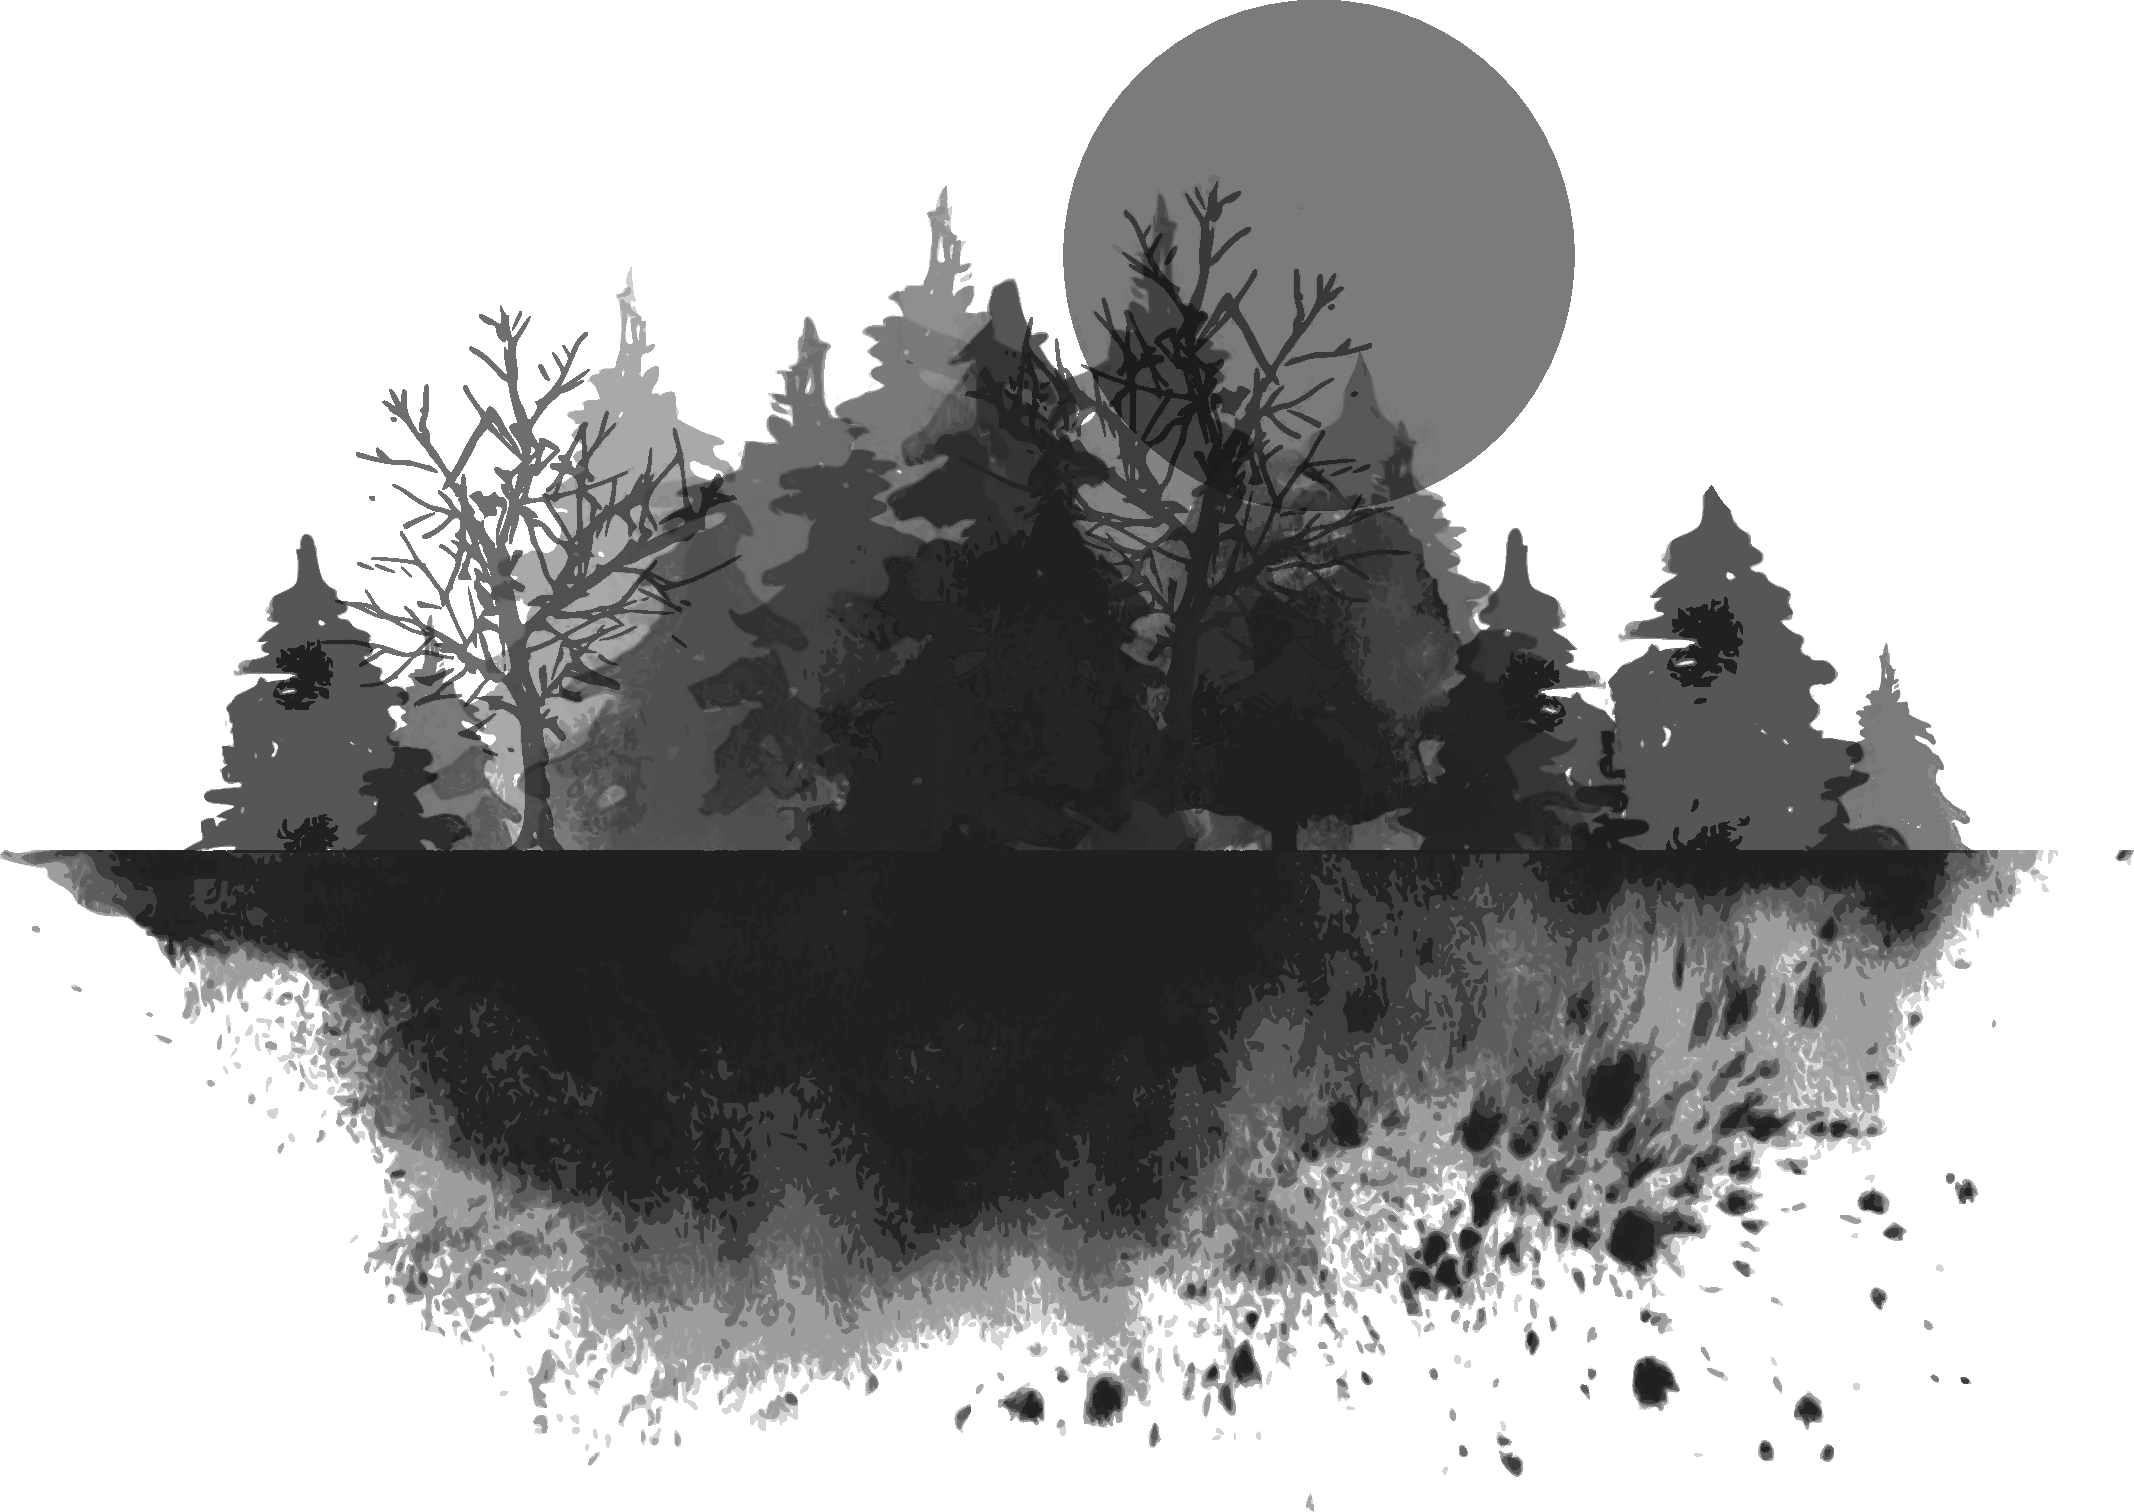
\includegraphics[scale=0.15]{Images/landscape.png}
\end{center}

\end{document}